\documentclass{article}
\usepackage{amsmath, amsfonts, amssymb}
\usepackage{graphicx}
\begin{document}

\section*{Understanding the Paradox:}

Stein's Paradox arises in the context of estimating multiple parameters simultaneously. The paradoxical finding by Charles Stein in 1956 was that, in three or more dimensions, there exist combined estimators that are better (in terms of mean squared error) than estimating each parameter individually, even when the individual estimations are unbiased and efficient for each parameter. This was contrary to the prevailing intuition derived from one-dimensional estimation problems.

\section*{Intuitive Explanation:}

\begin{enumerate}
    \item \textbf{Shrinkage Towards the Mean}: Imagine you're trying to estimate the abilities of multiple basketball players based on their performances. Instead of looking at each player's scoring average independently, Stein's estimator suggests that you can often make a better estimate for all players by slightly "shrinking" individual estimates toward the overall mean. This "shrinkage" can reduce the total error across all your estimates, especially when the players' performances are influenced by many common factors (like team strategies or opposition strength).
    \item \textbf{Borrowing Strength}: Stein's estimator effectively "borrows strength" from the other dimensions (or other parameters being estimated). When estimating multiple parameters, the information from one can inform and improve the estimate of the others. This is a fundamental concept in multivariate statistics, where the joint distribution of parameters can provide more information than considering each in isolation.
\end{enumerate}

\section*{Why It Only Works for \(d \geq 3\):}

\begin{enumerate}
    \item \textbf{Geometry of Higher Dimensions}: In one or two dimensions, the geometry doesn't allow for the kind of "borrowing strength" or pooling of information that is possible in three or more dimensions. It's related to how volumes and areas scale in higher dimensions and the nature of multivariate distributions. Essentially, as the number of dimensions increases, the proportion of the volume of a sphere that is close to the surface increases, allowing estimators to exploit the additional structure provided by the extra dimensions.
    \item \textbf{Mathematical Restrictions}: Mathematically, Stein's Paradox and the associated improvement in estimation do not manifest in one or two dimensions because the risk improvement term (which depends on the dimensionality of the problem) disappears or is not sufficient to overcome the estimation bias introduced.
\end{enumerate}

\section*{Conclusion:}

Stein's Paradox, through the lens of Stein's Estimator (or James-Stein Estimator), demonstrates that in higher-dimensional spaces (three or more dimensions), estimators can be constructed that outperform the traditional method of independently estimating each parameter. It's a result that has profound implications in statistical theory and practice, particularly in how we approach multivariate problems and the benefits of considering the structure and relationship between multiple pieces of data. This principle is widely used in modern statistical methods, including shrinkage techniques in high-dimensional data analysis and machine learning.

\begin{figure}
    \centering
    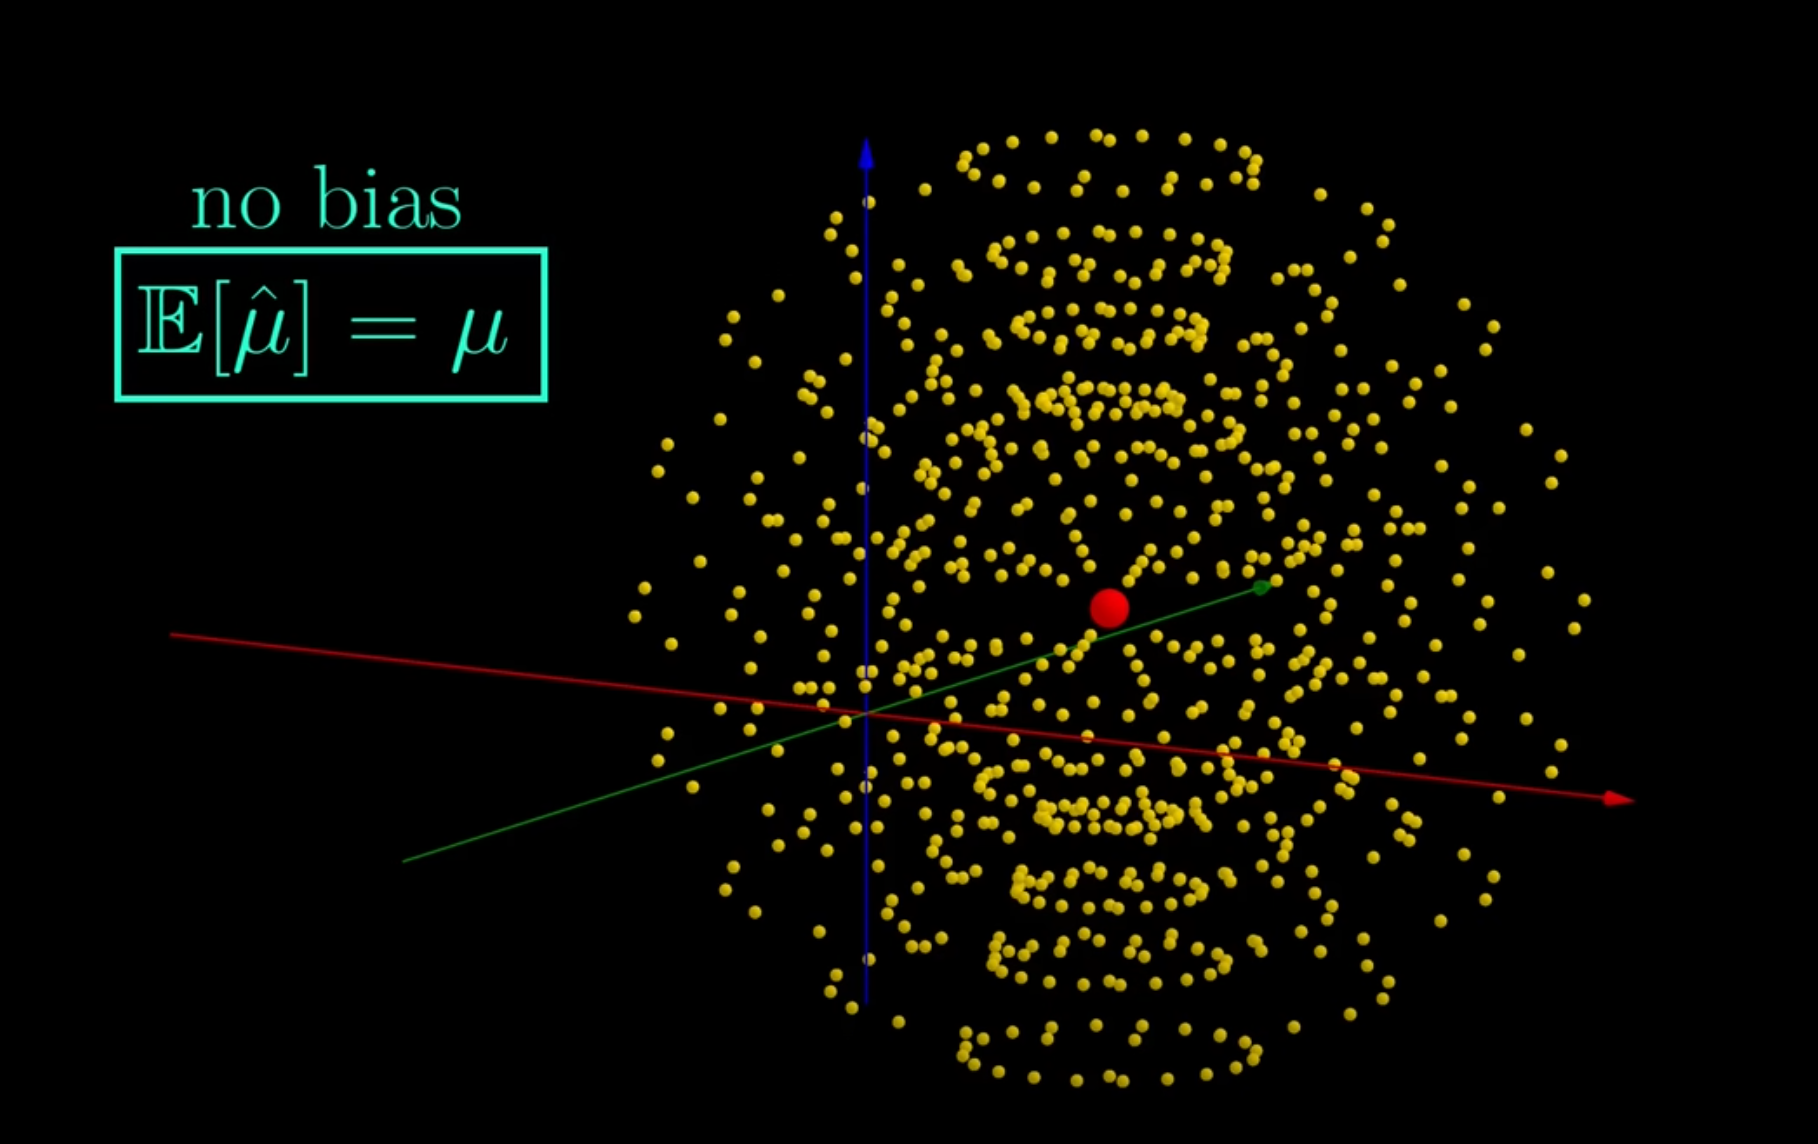
\includegraphics[width=1\linewidth]{overviews/james-stein-estimator/figures/unbiased.png}
    \caption{}
    \label{fig:enter-label}
\end{figure}
\begin{figure}
    \centering
    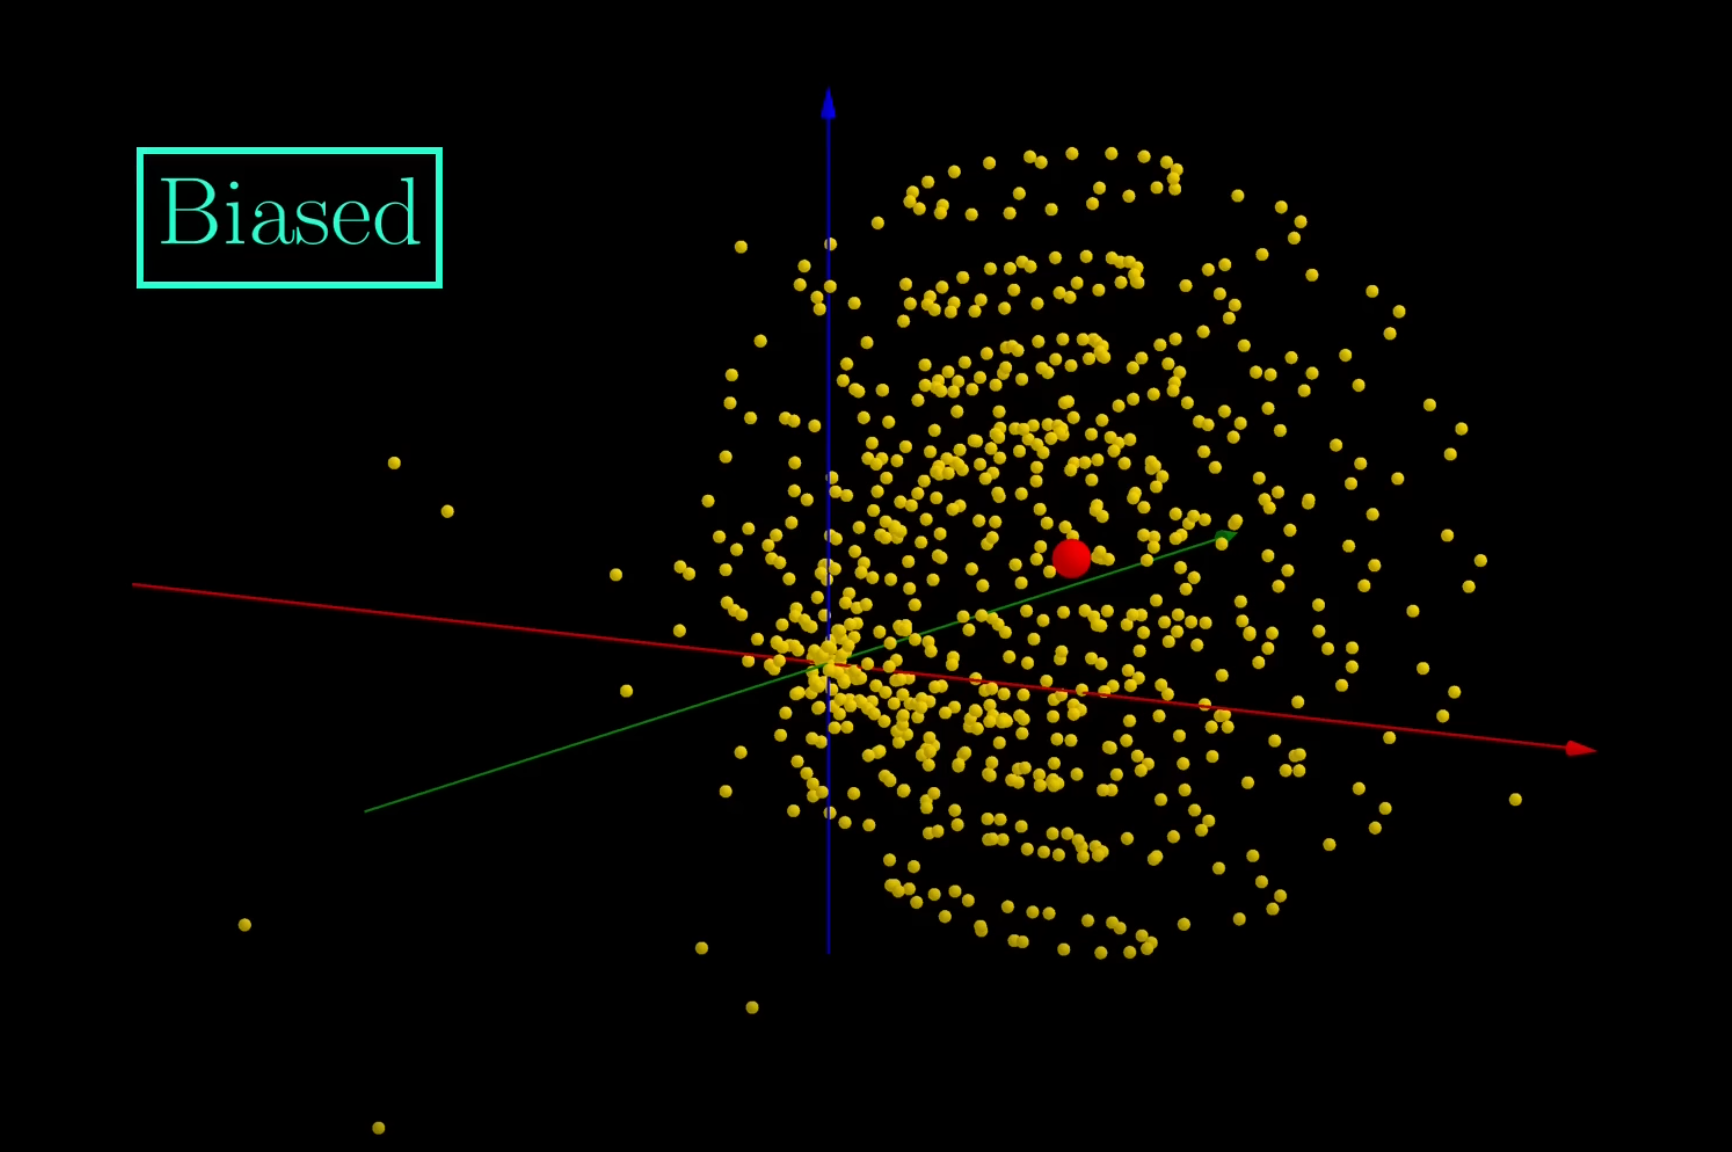
\includegraphics[width=1\linewidth]{overviews/james-stein-estimator/figures/biased.png}
    \caption{}
    \label{fig:enter-label}
\end{figure}

\section*{Mathematical Explanation of Stein's Paradox:}

To understand Stein's Paradox and the James-Stein estimator mathematically, let's start with a typical estimation problem. Suppose you have \(d\) normal distributions, each with unknown mean \(\theta_i\) and known variance \(\sigma^2\). Your goal is to estimate the vector of means \(\boldsymbol{\theta} = (\theta_1, \theta_2, ..., \theta_d)\) based on observed samples \(X_1, X_2, ..., X_d\).

\subsection*{Traditional Approach:}

The traditional approach would be to estimate each \(\theta_i\) independently using the sample mean of the corresponding distribution. This is the Maximum Likelihood Estimator (MLE) for normal distributions, which is unbiased and efficient in one-dimensional settings. So, you might estimate each mean by the corresponding sample mean \(X_i\).

\subsection*{Stein's Paradox in Estimation:}

Stein's Paradox suggests that, when \(d \geq 3\), you can construct an estimator that "shrinks" each \(X_i\) towards a common value (often towards the overall mean or zero) and overall produces a smaller mean squared error (MSE) than the individual estimators. This phenomenon occurs even if each \(X_i\) is an unbiased estimator of \(\theta_i\).

\subsection*{James-Stein Estimator:}

The James-Stein Estimator is a famous example that demonstrates this paradox. The estimator is given by:

\[
\hat{\boldsymbol{\theta}}_{JS} = \left(1 - \frac{(d-2) \sigma^2}{\|\boldsymbol{X}\|^2}\right) \boldsymbol{X}
\]

Where:

\begin{itemize}
    \item \(\boldsymbol{X} = (X_1, X_2, ..., X_d)\) is the vector of sample means.
    \item \(\|\boldsymbol{X}\|^2\) is the squared Euclidean norm of \(\boldsymbol{X}\).
    \item \(\sigma^2\) is the known variance of each observation.
\end{itemize}

\subsection*{Why the James-Stein Estimator Works Better for \(d \geq 3\):}

\begin{itemize}
    \item \textbf{Shrinkage Factor}: The term \(\left(1 - \frac{(d-2) \sigma^2}{\|\boldsymbol{X}\|^2}\right)\) is known as the shrinkage factor. It pulls the estimates towards zero (or towards the overall mean if you're centering your data). The amount of shrinkage increases as the sample means get closer to zero and decreases as they move away. This pooling of information leads to a lower MSE.
    \item \textbf{Bias vs. Variance Trade-off}: While the James-Stein Estimator introduces bias (since it's not unbiased like the individual \(X_i\)), it substantially reduces the variance of the estimate, particularly when the true means are close together. The overall effect is a decrease in MSE, which is a trade-off between bias and variance.
\end{itemize}

\begin{figure}
    \centering
    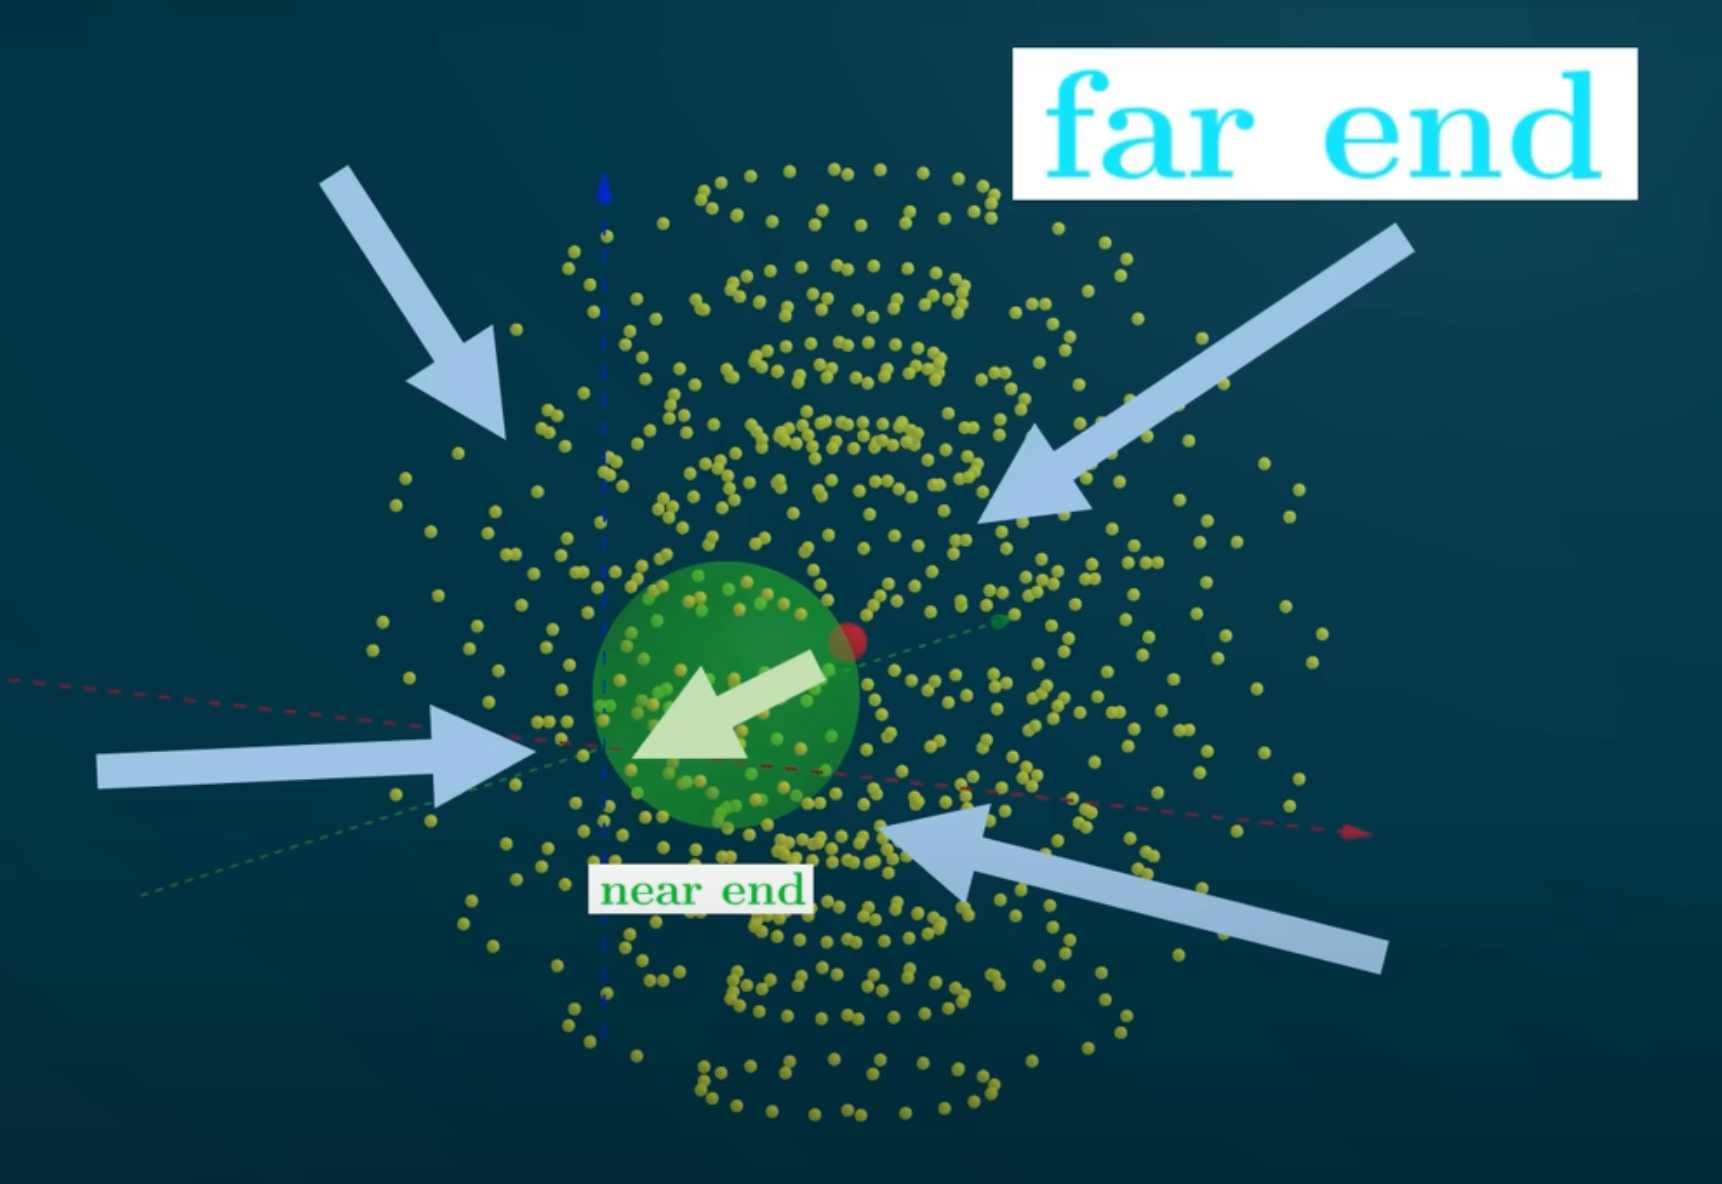
\includegraphics[width=1\linewidth]{overviews/james-stein-estimator/figures/near_far_end.png}
    \caption{Enter Caption}
    \label{fig:enter-label}
\end{figure}

\subsection*{Mathematical Implications:}

\begin{itemize}
    \item \textbf{Dominance over Traditional Estimators}: The James-Stein Estimator is said to dominate the traditional estimator (the sample means) in terms of mean squared error when \(d \geq 3\). This means it has a smaller MSE for every possible value of \(\boldsymbol{\theta}\) except for a set of measure zero.
    \item \textbf{Role of Dimensionality}: The paradox does not hold for \(d < 3\). This is tied to the geometry of higher-dimensional spaces, where there is more "room" to benefit from estimating parameters jointly rather than individually.
\end{itemize}

\end{document}

